\subsubsection{Overview}


\begin{figure}
\centering
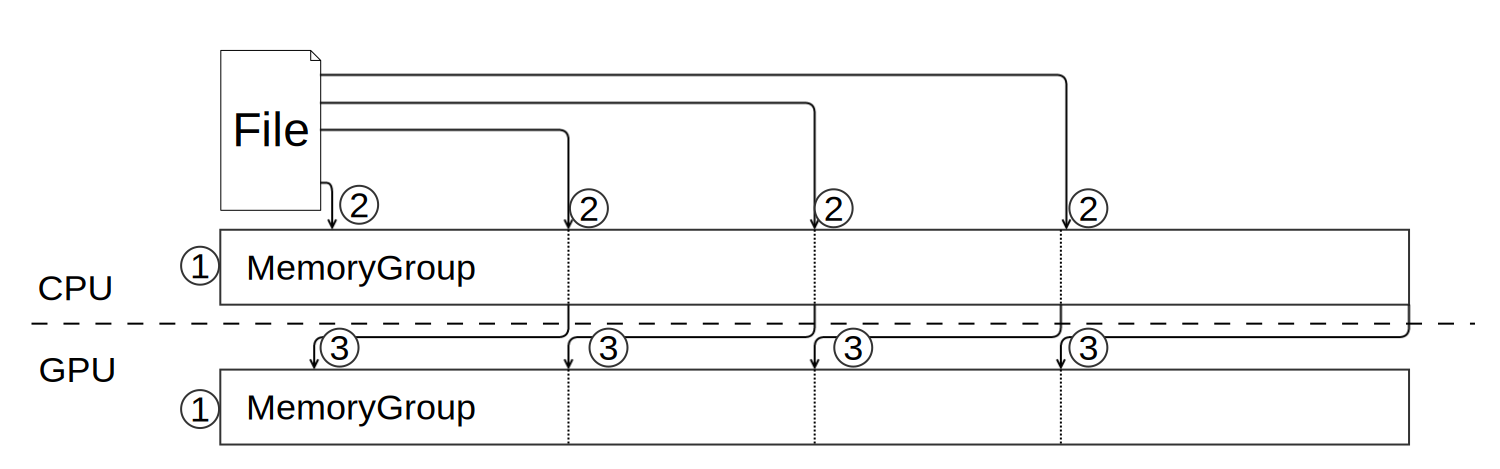
\includegraphics[scale=0.2]{fig/memory_group.pdf}
\caption{Memory Streaming Design}
\label{fig:memorygroup}
\centering
\end{figure}

The purpose of the runtime is two fold.
First, it simplifies our code generation --- alowing us to 
	have a unified view of memory and simplifying the 
	code generator.
Second, it eagerly copies data to the GPU.

The runtime does a few things to solve these problems.
To unify memory, we create a new object called \fix{zMemoryGroup\_t}
	this object contains multiple \fix{zMemory\_t} which 
	index into a contiguious array buffer for both CPU and GPU memories.
Each \fix{zMemory\_t} holds a state, such as
	\fix{unalloacted}, \fix{allocated},
	\fix{dirtyDevice}, etc\ldots
	that allow us to maintain conherence and avoid copies when
	not necessary.
The memory object also contain size and type information,
	and we operate on \fix{zMemory\_t} rather than a \fix{void *}
	types.
The abstract also facilitates us to other language supports, such 
	as OpenCL, without changing our code generator.

To eagerly copy memory to the GPU, we use logic similar to what is
	shown in figure~\ref{fig:memorygroup}.
In (1), we concurrently alloate CPU memory and GPU memory.
The file is then opened in (2) and different chunks are read into
	the CPU memory one it's been allocated (we \fix{mmap} the file
	with the \fix{PROT\_READ, MAP\_PRIVATE} options to increase
	performance).
Once a chunk of data is read, and GPU memory is allocate, data 
	is copied to the GPU in (3).
Note that while we have independent view of chunks of memory 
	(defined by the datatype \fix{zMemory\_t}) memory is in fact
	contiguious and placed in a \fix{zMemoryGroup\_t} object.
This makes it possible to free memory efficiently, and, althought
	not presently implemented, allows us to resize the chunk
	sizes.
